
\section{Factory Language (.fl)}\label{appendix:factory-lang}

\subsection{Metamodel}\label{appendix:metamodel} 

\begin{figure}[H]
    \centering
    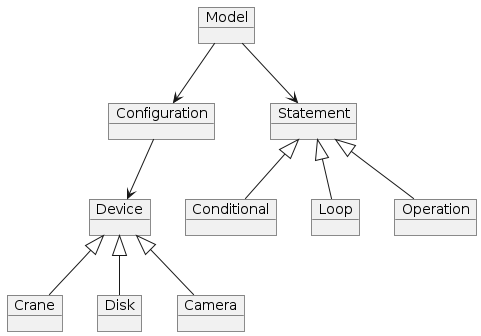
\includegraphics[width=.40\textwidth]{Image/metamodel-final.png}
    \caption{An overview of the metamodel.}
    \label{fig:metamodel}
\end{figure}

\subsection{Grammar Language}\label{appendix:grammar-language}

\begin{minted}[breaklines]{python}
grammar xtext.factoryLang.FactoryLang with org.eclipse.xtext.common.Terminals

generate factoryLang "http://www.factoryLang.xtext/FactoryLang"

Model:
	configurations+=Configuration+ statements+=Statement+;

// ----- CONFIGURATION ----- //
Configuration:
	'create' device=Device;

Device:
	Crane | Disk | Camera;

// ----- CONFIGURATION:CRANE ----- //
Crane returns Device:
	{Crane} 'crane' 'named' name=ID BEGIN targets+=CraneParameter+ END;

CraneParameter returns Parameter:
	CranePositionParameter;

CranePositionParameter returns CraneParameter:
	{CranePositionParameter} 'with' 'position' 'at' degree=INT 'named' name=ID;

// ----- CONFIGURATION:DISK ----- //
Disk returns Device:
	{Disk} 'disk' 'named' name=ID BEGIN slotParameter=DiskSlotParameter targets+=DiskParameter+ END;

DiskParameter returns Parameter:
	DiskZoneParameter;

DiskSlotParameter returns DiskParameter:
	{DiskSlotParameter} 'with' size=INT 'slots';

DiskZoneParameter returns DiskParameter:
	{DiskZoneParameter} 'with' 'zone' 'named' name=ID 'at' 'slot' slot=INT;

// ----- CONFIGURATION:CAMERA ----- //
Camera returns Device:
	{Camera} 'camera' 'named' name=ID BEGIN targets+=CameraParameter+ END;

CameraParameter returns Parameter:
	CameraColorParameter;

CameraColorParameter returns CameraParameter:
	{CameraColorParameter} 'with' 'scannable' 'color' color=COLOR;

// ----- STATEMENTS ----- //
Statement:
	Conditional | Operation | Loop;

// ----- STATEMENTS:CONDITIONALS ----- //
Conditional returns Statement:
	DeviceConditional | VariableConditional;

DeviceConditional returns Conditional:
	{DeviceConditional} 'if' 'device' device=[Device] 'is' (not_operator='not')? ('at')?
	deviceValue=DeviceValue
	'then' BEGIN statements+=Statement* END;

VariableConditional returns Conditional:
	{VariableConditional} 'if' 'variable' variable=[Variable] 'is'
	(comparison_operator=COMPARISON_OPERATOR)?
	variableValue=VariableValue
	'then' BEGIN statements+=Statement* END;

// ----- STATEMENTS:OPERATIONS ----- //
Operation returns Statement:
	CraneOperation | DiskOperation | CameraOperation;

// ----- STATEMENTS:OPERATIONS:CRANE ----- //
CraneOperation returns Operation:
	CranePickupOperation | CraneDropOperation;

CranePickupOperation returns CraneOperation:
	{CranePickupOperation} device=[Crane] 'pickup' 'item' 'at' target=[CraneParameter];

CraneDropOperation returns CraneOperation:
	{CraneDropOperation} device=[Crane] 'drop' 'item' 'at' target=[CraneParameter];

// ----- STATEMENTS:OPERATIONS:DISK ----- //
DiskOperation returns Operation:
	DiskMoveEmptySlotOperation | DiskMoveVariableSlotOperation | DiskMoveSlotOperation | DiskMarkSlotOperation;

DiskMoveSlotOperation returns DiskOperation:
	{DiskMoveSlotOperation} device=[Disk] 'move' 'slot' 'at' source=[DiskZoneParameter] 'to'
	target=[DiskZoneParameter];

DiskMoveVariableSlotOperation returns DiskOperation:
	{DiskMoveVariableSlotOperation} device=[Disk] 'move' 'slot' 'of' variable=[Variable] 'to'
	target=[DiskZoneParameter];

DiskMoveEmptySlotOperation returns DiskOperation:
	{DiskMoveEmptySlotOperation} device=[Disk] 'move' 'empty' 'slot' 'to' target=[DiskZoneParameter];

DiskMarkSlotOperation returns DiskOperation:
	{DiskMarkSlotOperation} device=[Disk] 'mark' 'slot' 'at' target=[DiskZoneParameter] 'as'
	diskSlotValue=DiskSlotValue ('in' quantity=INT measure=TIME)?;

// ----- STATEMENTS:OPERATIONS:CAMERA ----- //
CameraOperation returns Operation:
	CameraScanOperation;

CameraScanOperation returns CameraOperation:
	{CameraScanOperation} device=[Camera] 'scan' 'color' 'into' variable=GlobalVariable;

// ----- STATEMENTS:LOOPS ----- //
Loop returns Statement:
	ForEach;

// ----- STATEMENTS:LOOPS:FOREACH ----- //
ForEach returns Loop:
	{ForEach} 'for' 'each' variable=LocalVariable 'in' device=[Device] 'that' 'is' (operator='not')?
	variableValue=VariableValue
	'then' BEGIN statements+=Statement* END;

// ----- VARIABLES ----- //
LocalVariable returns Variable:
	{LocalVariable} name=ID;

GlobalVariable returns Variable:
	{GlobalVariable} name=ID;

// ----- VALUE TYPES ----- //
DeviceValue:
	value=DiskStateValue | value=ColorValue | ref=[Parameter];

DiskSlotValue:
	value=DiskSlotStateValue | value=ColorValue | ref=[Variable];

VariableValue:
	value=DiskSlotStateValue | value=ColorValue | value=Number | value=DiskStateValue | ref=[Variable];

// ----- VALUE TYPES:ACTUAL VALUES ----- //

DiskStateValue:
	value=DISK_STATES;

DiskSlotStateValue:
 	value=DISK_SLOT_STATES;

ColorValue:
	value=COLOR;

Number:
	value=INT;

// ----- SHARED ENUMS ----- //
enum COMPARISON_OPERATOR:
	UNDEFINED='undefined' | LESS_THAN='less than' | GREATER_THAN='greater than' | NOT='not';

enum COLOR:
	RED='red' | GREEN='green' | BLUE='blue';

enum DISK_SLOT_STATES:
	FREE='free' | IN_PROGRESS='in_progress' | COMPLETE='complete';

enum DISK_STATES:
	FULL='full' | EMPTY='empty';

enum TIME:
	SECONDS='seconds' | SECOND='second' | MINUTES='minutes' | MINUTE='minute' | HOURS='hours' | HOUR='hour';

// ----- TERMINALS ----- //
terminal BEGIN:
	'synthetic:BEGIN';

terminal END:
	'synthetic:END';
\end{minted}

\subsection{Example Factory Language program}\label{appendix:fl}
\begin{minted}[breaklines]{python}
create crane named crane1  
	with position at 0 named pickup 
	with position at 30 named outRed 
	with position at 60 named outGreen 
	with position at 90 named outBlue  

create disk named disk1
	with 8 slots
	with zone named craneZone  at slot 1 
	with zone named cameraZone at slot 3 
	with zone named intakeZone at slot 6 

create camera named camera1  
	with scannable color blue 
	with scannable color green 
	with scannable color red

for each diskSlot in disk1 that is complete then
	disk1 move slot of diskSlot to craneZone
	crane1 pickup item at pickup
	if variable diskSlot is red then  
		crane1 drop item at outRed
	if variable diskSlot is green then  
		crane1 drop item at outGreen
	if variable diskSlot is blue then  
		crane1 drop item at outBlue
	disk1 mark slot at craneZone as free

if device disk1 is not full then  
	disk1 move empty slot to intakeZone
	disk1 mark slot at intakeZone as in_progress 
	disk1 move slot at intakeZone to cameraZone
	camera1 scan color into currentItemColor 
	disk1 mark slot at cameraZone as currentItemColor  
	if variable currentItemColor is red then  
		disk1 mark slot at cameraZone as complete in 10 seconds
	if variable currentItemColor is green then  
		disk1 mark slot at cameraZone as complete in 20 seconds  
	if variable currentItemColor is blue then  
		disk1 mark slot at cameraZone as complete in 30 seconds
\end{minted}
